%%%%%%%%%%%%%%%%%%%%%%%%%%%%%%%%%%%%%%%%%
% University/School Laboratory Report
% LaTeX Template
% Version 3.1 (25/3/14)
%
% This template has been downloaded from:
% http://www.LaTeXTemplates.com
%
% Original author:
% Linux and Unix Users Group at Virginia Tech Wiki 
% (https://vtluug.org/wiki/Example_LaTeX_chem_lab_report)
%
% License:
% CC BY-NC-SA 3.0 (http://creativecommons.org/licenses/by-nc-sa/3.0/)
%
%%%%%%%%%%%%%%%%%%%%%%%%%%%%%%%%%%%%%%%%%

%----------------------------------------------------------------------------------------
%	PACKAGES AND DOCUMENT CONFIGURATIONS
%----------------------------------------------------------------------------------------

%\documentclass[12pt]{article}
\documentclass[14pt]{extarticle}

\usepackage{setspace} % For set space
\usepackage{algorithm} % For pseudo code
\usepackage[noend]{algpseudocode}
\usepackage{siunitx} % Provides the \SI{}{} and \si{} command for typesetting SI units
\usepackage{graphicx} % Required for the inclusion of images
\usepackage{natbib} % Required to change bibliography style to APA
\usepackage{amsmath} % Required for some math elements 

%\setlength\parindent{0pt} % Removes all indentation from paragraphs

\renewcommand{\labelenumi}{\alph{enumi}.} % Make numbering in the enumerate environment by letter rather than number (e.g. section 6)
\renewcommand{\baselinestretch}{1.5}
%\usepackage{times} % Uncomment to use the Times New Roman font

%----------------------------------------------------------------------------------------
%	DOCUMENT INFORMATION
%----------------------------------------------------------------------------------------

\title{\large Multiple AI Competition in Self Developed Game \\ Term 1 Report \\ ESTR4998/4999} % Title

\date{\today} % Date for the report

\begin{document}


\maketitle % Insert the title, author and date

\begin{center}
\begin{tabular}{l r}
Partners: & XIAO Tianyi \\ % Partner names
& LUO Lu \\
Instructor: & Prof. Andrej Bogdanov % Instructor/supervisor
\end{tabular}
\end{center}
\newpage
% If you wish to include an abstract, uncomment the lines below
\begin{abstract}
% Abstract text
\end{abstract}

%----------------------------------------------------------------------------------------
%	SECTION 1
%----------------------------------------------------------------------------------------

\section{Abstract}

To determine the atomic weight of magnesium via its reaction with oxygen and to study the stoichiometry of the reaction (as defined in \ref{definitions}):


% If you have more than one objective, uncomment the below:
%\begin{description}
%\item[First Objective] \hfill \\
%Objective 1 text
%\item[Second Objective] \hfill \\
%Objective 2 text
%\end{description}

\subsection{Definitions}
\label{definitions}
\begin{description}
\item[Stoichiometry]
The relationship between the relative quantities of substances taking part in a reaction or forming a compound, typically a ratio of whole integers.
\item[Atomic mass]
The mass of an atom of a chemical element expressed in atomic mass units. It is approximately equivalent to the number of protons and neutrons in the atom (the mass number) or to the average number allowing for the relative abundances of different isotopes. 
\end{description} 
 
%----------------------------------------------------------------------------------------
%	SECTION 2
%----------------------------------------------------------------------------------------

\section{Background}

\subsection{Related Works}

\subsection{Tensorflow}

\subsection{Pygame}

\begin{tabular}{ll}
Mass of empty crucible & \SI{7.28}{\gram}\\
Mass of crucible and magnesium before heating & \SI{8.59}{\gram}\\
Mass of crucible and magnesium oxide after heating & \SI{9.46}{\gram}\\
Balance used & \#4\\
Magnesium from sample bottle & \#1
\end{tabular}

%----------------------------------------------------------------------------------------
%	SECTION 3
%----------------------------------------------------------------------------------------

\section{Introduction}

\subsection{Game Development Platform}
Considering the training process of AI, a game platform based on Python would be more suitable than other main stream game development platforms nowadays, like Unity or Unreal Engine 4. Therefore, we choose Pygame as our game development platform.

%----------------------------------------------------------------------------------------
%	SECTION 4
%----------------------------------------------------------------------------------------

\section{Design}

The design of our FYP is based on two parts, which are the game part and AI part.

\subsection{Game Design}

\subsubsection{Game Mode}
In consideration of the cost of game development, basically the time cost, we decide to implement a game with straightforward structure. For the purpose of AI training, the game should have one clear goal and controllable user inputs, otherwise the workload and cost of the FYP could be hard to measure. Then as the result of teamwork discussion, soccer game is chosen as the game mode.

\subsubsection{Game Rule}
\begin{description}
	\item[Team and players]
	There are two teams (team-0 and team-1) in the game. For each team, ther are N players (1 $\leq$ N $\leq$ 7).
	\item[Goal]
	If a ball pass through the goal of a team, then opposite team would get a score. And in each turn of the game, the team who get most scores will win the game, otherwise it ends in a draw. Therefore, for each team, they should try their best to get more scores and prevent the opposite team to get any score.
	\item[time]
	Every turn of game has a time limit. As soon as it reaches time limit, this turn of game will be forcely over.
\end{description}

\subsubsection{Player Action}
For each player, it can get the ball when it is free, steal the ball when it is catched by another player, and shoot the ball when it is catching the ball.
\begin{description}
	\item[catch]
	When a ball is not catched by any player, any player can try to get the ball. As soon as a player touch the ball, the player will get the ball.
	\item[Steal]
	When a ball is catched by a player, other players can steal the ball from player. As long as another player touch the player with ball, the ball would be stolen. However, after a player just get the ball, there will be a short invincible period. Only after the invincible period, can other players steal the ball.
	\item[shoot]
	When a player is catching the ball, the player can shoot the ball away. It can shoot the ball along the eight directions, which are left, right, up, down, upper-left, upper-right, lower-left, lower-right.\\
	And for the player just shoot the ball, it need to wait for a short period to be able to get the ball again.
\end{description}

\subsubsection{Other Details About Game}
\begin{description}
	\item[boundary]
	When the ball reach the boundary, it will bounce back. Players are not able to get out of boundary.
	\item[Initialization and Reset]
	When each turn of game begins, every player would be assigned to an initial position, and ball will be placed in the center of the field. And when any of two teams get a score, the positions of players and ball will also be reset to initial positions.
\end{description}

\subsection{AI Design}


%----------------------------------------------------------------------------------------
%	SECTION 5
%----------------------------------------------------------------------------------------

\section{Implement}

\subsection{Game Implementation}

In our pygame implementation of the soccer game, we build two important classes \textbf{Player} and \textbf{Ball}.

\subsubsection{Player}
The Player class inherits from Sprite, which is a pre-defined class of pygame module. Below are methods of Player.
\begin{description}
	\item[\_\_init\_\_]
	In the \_\_init\_\_ method, we define and initialize the related variavles of a player, assign an id and initial position to the player, and load the image of players.
	\begin{figure}[H]
		\begin{center}
			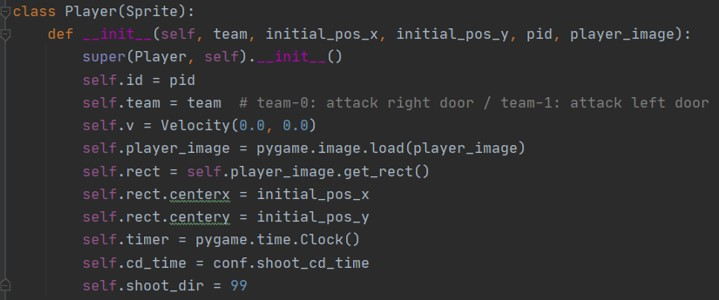
\includegraphics[width=0.9\textwidth]{Player_init}
			\caption{implementation of \_\_init\_\_ in Player}
		\end{center}
	\end{figure}
	\item[input\_handler]
	In the input\_handler, an input array is passed into the method. The input array contains information about user input, including the four moving directions along x and y axes, and if the user want shoot the ball. If no user input on one axis, or two opposite directions (like up and down, or left and right) show up at the same time, the player will not have velocity on that axis. Otherwise, the velocity will be added on the corresponding directions. If the user want to shoot the ball, the related shoot\_dir will be calculated through xy\_to\_dir, and then be dealt with if the ball belongs to this player.
	\begin{figure}[H]
		\begin{center}
			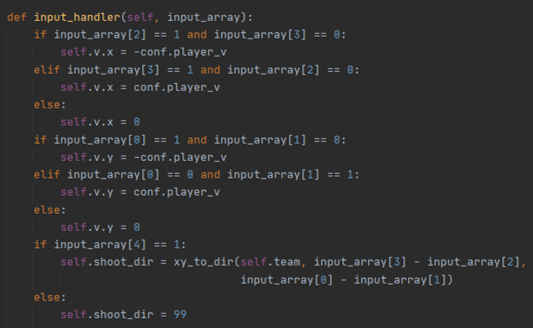
\includegraphics[width=0.9\textwidth]{Player_input}
			\caption{implementation of init\_handler in Player}
		\end{center}
	\end{figure}
	\begin{figure}[H]
	\begin{center}
			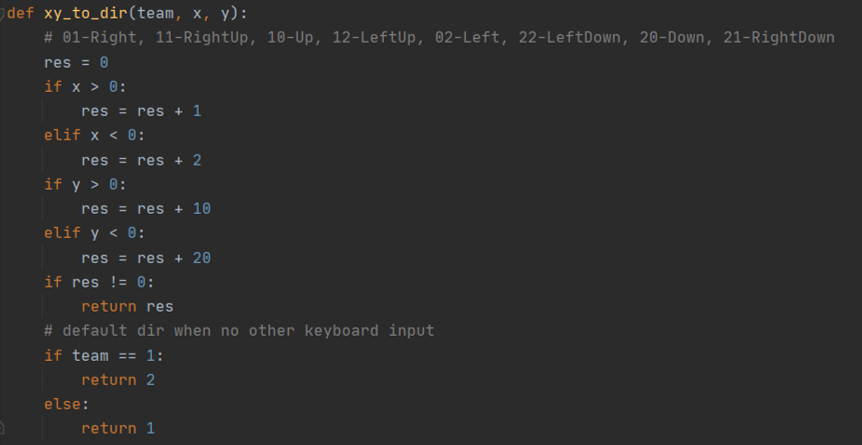
\includegraphics[width=0.9\textwidth]{xy_to_dir}
			\caption{implementation of xy\_to\_dir}
		\end{center}
	\end{figure}
	\item[update]
	In the update, the position of a player would be updated according to its velocity. And boundary check will be executed, in case that the player cross over the boundary. 
	\begin{figure}[H]
		\begin{center}
			\includegraphics[width=0.9\textwidth]{Player_update}
			\caption{implementation of update in Player}
		\end{center}
	\end{figure}
	\item[shoot\_update]
	In shoot\_update, after player shoot the ball, the timer will tick, for check\_shoot\_cd to check time.
	\begin{figure}[H]
		\begin{center}
			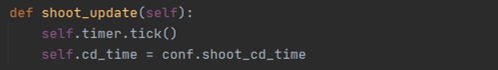
\includegraphics[width=0.9\textwidth]{Player_shoot_update}
			\caption{implementation of shoot\_update in Player}
		\end{center}
	\end{figure}
	\item[check\_shoot\_cd]
	If a player want to get the ball, the system will check if it just shoot the ball by using the timer, which begins to tick in shoot\_update.
	\begin{figure}[H]
		\begin{center}
			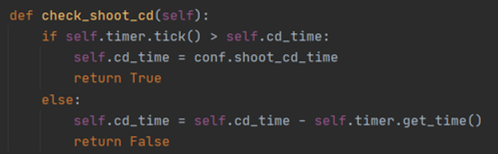
\includegraphics[width=0.9\textwidth]{Player_check_shoot_cd}
			\caption{implementation of cehck\_shoot\_cd\_time in Player}
		\end{center}
	\end{figure}
	\item[render]
	In render, the update function will be called. Then the player will be rendered through the screen, which is passed to the render method.
	\begin{figure}[H]
		\begin{center}
			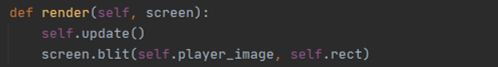
\includegraphics[width=0.9\textwidth]{Player_render}
			\caption{implementation of render in Player}
		\end{center}
	\end{figure}
\end{description}

\subsubsection{Ball}
The Ball class inherits from Sprite, which is a pre-defined class of pygame module. Below are methods of Ball.
\begin{description}
	\item[\_\_init\_\_]
	In the \_\_init\_\_ method, we define and initialize the related variavles of the ball, assign initial position to the player, and load the image of players.
	\begin{figure}[H]
		\begin{center}
			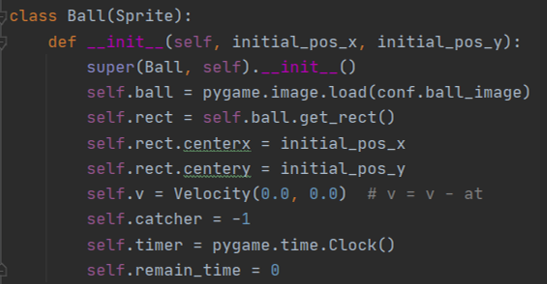
\includegraphics[width=0.9\textwidth]{Ball_init}
			\caption{implementation of \_\_init\_\_ in Ball}
		\end{center}
	\end{figure}
	\item[belong]
	In the belong, an player id is passed into this method, and it will be checked that if the ball belongs to the player with this id. 
	\begin{figure}[H]
		\begin{center}
			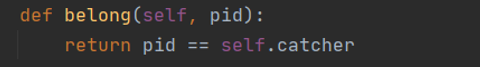
\includegraphics[width=0.9\textwidth]{Ball_belong}
			\caption{implementation of belong in Ball}
		\end{center}
	\end{figure}
	\item[caught]
	In the caught, the ball is caught by the player with given player id. And the information about tha ball would be updated.
	\begin{figure}[H]
		\begin{center}
			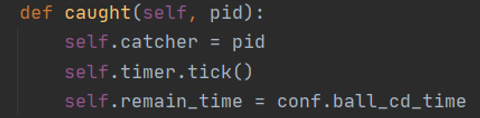
\includegraphics[width=0.9\textwidth]{Ball_caught}
			\caption{implementation of caught in Ball}
		\end{center}
	\end{figure}
	\item[copy\_pos]
	Position of ball will be updated according to the x and y value passed.
	\begin{figure}[H]
		\begin{center}
			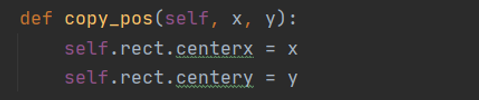
\includegraphics[width=0.9\textwidth]{Ball_copy_pos}
			\caption{implementation of copy\_pos in Ball}
		\end{center}
	\end{figure}
	\item[check\_time\_up]
	In check\_time\_up, the remain time of invincible period will be checked. If the invincible time is up, the method will return True, which means other players can steal the ball from the player catching the ball.
	\begin{figure}[H]
		\begin{center}
			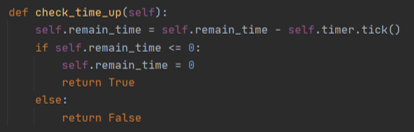
\includegraphics[width=0.9\textwidth]{Ball_check_time}
			\caption{implementation of check\_time\_up in Ball}
		\end{center}
	\end{figure}
	\item[shoot\_ball]
	Update relative information of the ball, after a player shoot the ball, and update velocity of the ball through dir\_to\_xy.
	\begin{figure}[H]
		\begin{center}
			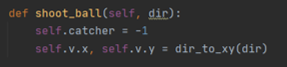
\includegraphics[width=0.9\textwidth]{Ball_shoot}
			\caption{implementation of shoot\_ball in Ball}
		\end{center}
	\end{figure}
	\begin{figure}
		\begin{center}
			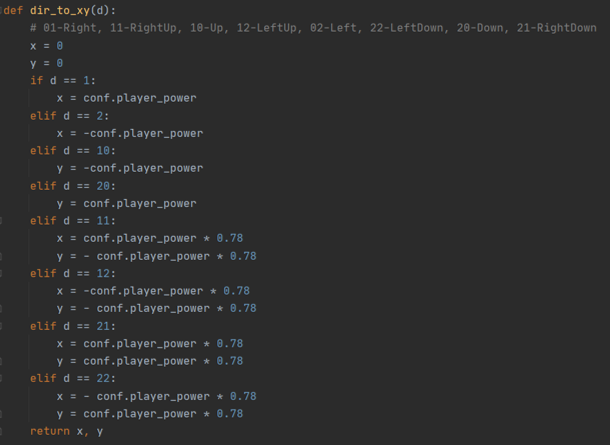
\includegraphics[width=0.9\textwidth]{dir_to_xy}
			\caption{implementation of dir\_to\_xy}
		\end{center}
	\end{figure}
	\item[update\_pos]
	In update\_pos, position of ball will be updated according to it velocity, and boundary rebounce will be done. Also, the velocity will also be updated, according to the friction of the ground through update\_v.
	\begin{figure}[H]
		\begin{center}
			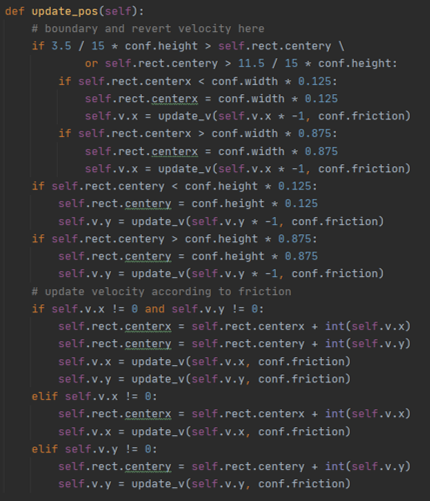
\includegraphics[width=0.9\textwidth]{Ball_update_pos}
			\caption{implementation of update\_pos in Ball}
		\end{center}
	\end{figure}
	\begin{figure}[H]
		\begin{center}
			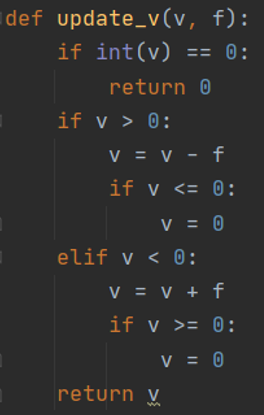
\includegraphics[width=0.3\textwidth]{update_v}
			\caption{implementation of update\_v}
		\end{center}
	\end{figure}
	\item[render]
	In render, update\_pos is called. Then, ball is rendered through the screen passed to this method.
	\begin{figure}[H]
		\begin{center}
			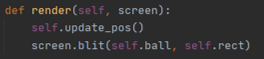
\includegraphics[width=0.9\textwidth]{Ball_render}
			\caption{implementation of render in Ball}
		\end{center}
	\end{figure}
	\item[in\_door]
	In this function, it is checked that if any team get a score. If team-0 get a score, return 0, if team-1 get a score, return 1. Otherwise, return -1.
	\begin{figure}[H]
		\begin{center}
			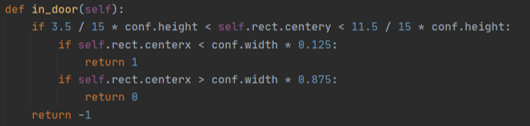
\includegraphics[width=0.9\textwidth]{Ball_in_door}
			\caption{implementation of in\_door in Ball}
		\end{center}
	\end{figure}
\end{description}

\subsubsection{Main Part}
	First, information about the game is initialized, and important variables storing information about the game are built. Here a function named initialuze\_game will be called.
	\begin{figure}[H]
	\begin{center}
		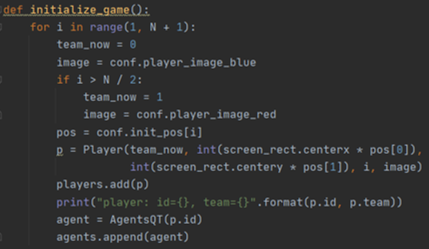
\includegraphics[width=0.9\textwidth]{initialize_game}
		\caption{implementation of initialize\_game}
	\end{center}
	\end{figure}
	In the main while loop of game execution, first each player will deal with its input passed from AI, through the relative method of Player and Ball.
	\begin{figure}[H]
	\begin{center}
		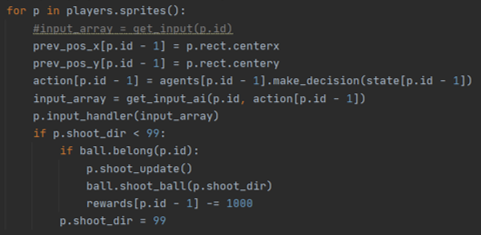
\includegraphics[width=0.9\textwidth]{deal_with_input}
		\caption{implementation of main part about dealing with input}
	\end{center}
	\end{figure}
	Then, the system will detect if there is any collision between player and ball, and judge if any player get or steal the ball according to the state of ball and the player catching the ball (if any). Then position of the ball will be updated, and sysytem will check if any team get a score. 
	\begin{figure}[H]
	\begin{center}
		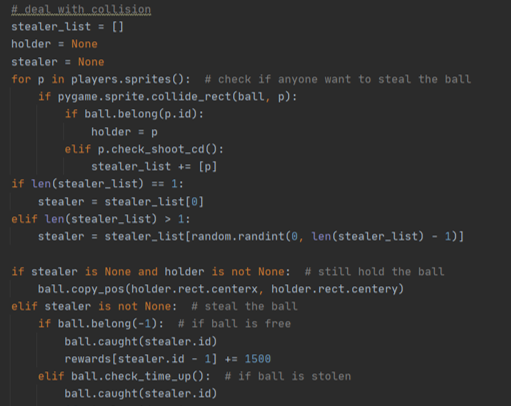
\includegraphics[width=0.9\textwidth]{collision}
		\caption{implementation of main part about collision}
	\end{center}
	\end{figure}
	Finally, iamge of every player and ball will be rendered un the screen.
	\begin{figure}[H]
		\begin{center}
			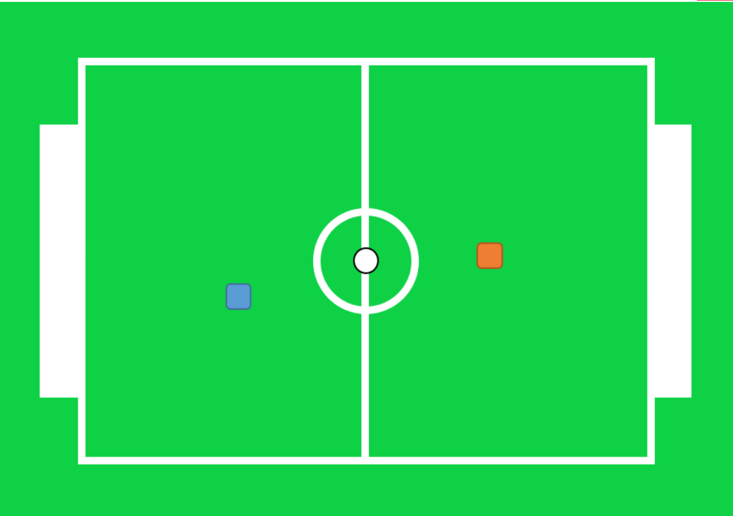
\includegraphics[width=0.9\textwidth]{game}
			\caption{Game}
		\end{center}
	\end{figure}

\subsection{AI Implementation}
	
	
%----------------------------------------------------------------------------------------
%	SECTION 6
%----------------------------------------------------------------------------------------

\section{Current Conclusion}

\begin{enumerate}
\begin{item}
The \emph{atomic weight of an element} is the relative weight of one of its atoms compared to C-12 with a weight of 12.0000000$\ldots$, hydrogen with a weight of 1.008, to oxygen with a weight of 16.00. Atomic weight is also the average weight of all the atoms of that element as they occur in nature.
\end{item}
\begin{item}
The \emph{units of atomic weight} are two-fold, with an identical numerical value. They are g/mole of atoms (or just g/mol) or amu/atom.
\end{item}
\begin{item}
\emph{Percentage discrepancy} between an accepted (literature) value and an experimental value is
\begin{equation*}
\frac{\mathrm{experimental\;result} - \mathrm{accepted\;result}}{\mathrm{accepted\;result}}
\end{equation*}
\end{item}
\end{enumerate}

%----------------------------------------------------------------------------------------
%	SECTION 5
%----------------------------------------------------------------------------------------

\section{Future Plan}

placeholder

The most obvious source of experimental uncertainty is the limited precision of the balance. Other potential sources of experimental uncertainty are: the reaction might not be complete; if not enough time was allowed for total oxidation, less than complete oxidation of the magnesium might have, in part, reacted with nitrogen in the air (incorrect reaction); the magnesium oxide might have absorbed water from the air, and thus weigh ``too much." Because the result obtained is close to the accepted value it is possible that some of these experimental uncertainties have fortuitously cancelled one another.

%----------------------------------------------------------------------------------------
%	BIBLIOGRAPHY
%----------------------------------------------------------------------------------------

\bibliographystyle{apalike}

\bibliography{sample}

%----------------------------------------------------------------------------------------


\end{document}